
A number of diagnostic measurements were made for each particle to find possible problems with the setup. We only show the diagnostic measurements from measurement 1 in this section but all plots can be found at \url{http://goo.gl/jgzSXe}.


\begin{figure}[H]
\begin{center}
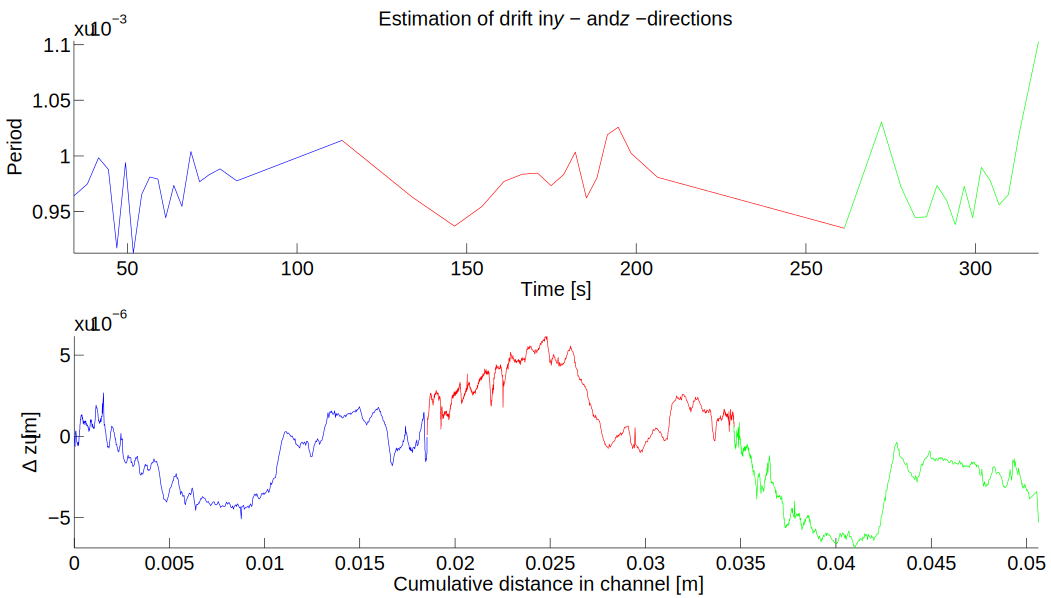
\includegraphics[width=0.7\textwidth]{figures/results/particleA/October_11_Particle_2_run_2_B.pdf}
\end{center}
\caption{The estimation of drift in $y$ and $z$ direction for Particle from measurement 1. Upper figure is the estimation of the sinking of the particle, the lower figure is the measured z position in the channel against cumulative distance. }
\label{fig:particleAsink}
\end{figure}

\begin{figure}[H]
\centering
\includegraphics[width=0.7\textwidth]{figures/results/particleB/October_1_Particle_4_run_4_B.pdf}	
\caption{The estimation of drift in $y$ and $z$ direction for Particle from measurement 1. Upper figure is the estimation of the sinking of the particle, the lower figure is the measured z position in the channel against cumulative distance.}
\label{fig:particleB2sinking}
\end{figure}



The center of mass movement in the direction perpendicular to the flow direction $x$ is seen in Figures \ref{fig:particleAsink} and \ref{fig:particleB2sinking}. Movement in the $y$ direction, i.e. sinking or floating, was measured by plotting the period of each flip against time as in the upper graph of figure  The period here refers to the distance $\Delta_i$ between two successive zeros for $n_x$ relative to the first such distance $\Delta_0$. If there is no clear trend to higher or lower values it implies that there is little sinking or floating. 

The movement in the z coordinate is very small relative to the movements in the x direction. We can see that Z-direction movements along one stretch are on the order of $10\mu m$ compared to the x direction which is on the order of $2\cdot 10^4 \mu m$.The change in period was less than 20\% for all particles presented in this section.

The speed was plotted as a function of time to see how the flow reversed and if there were any problems with the pump. There is a noticeable difference between reversals that occur on the side of the channel and the side closer to the pump where on the reversal on the end of the channel further from the pump the speed drops to 0, increases for a short while and then goes back down to 0. This has been a consistent feature across all measurements.

\begin{figure}[H]
\begin{center}
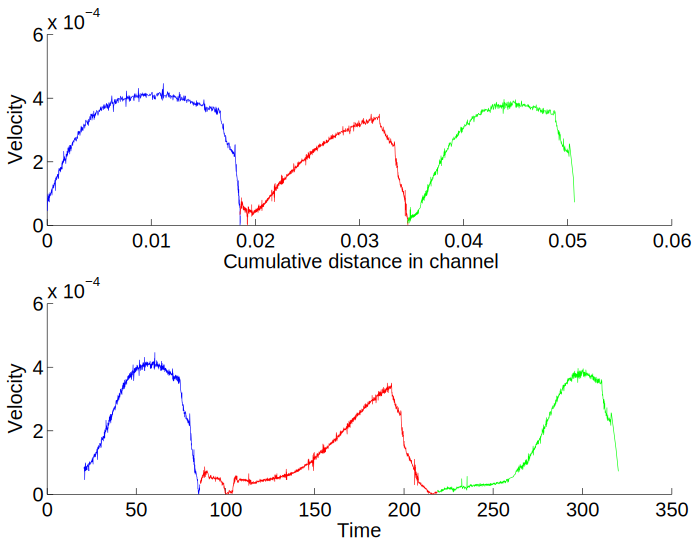
\includegraphics[width=0.7\textwidth]{figures/results/particleA/October_11_Particle_2_run_2_D.pdf}
\end{center}
\caption{The speed (note not the velocity) of the particle A from measurement 1 against cumulative distance in the upper figure and against time in the lower figure.}
\label{fig:particleAspeed}
\end{figure}


\begin{figure}[H]
\begin{center}
\includegraphics[width=0.7\textwidth]{figures/results/particleB/October_1_Particle_4_run_2_D.pdf}
\end{center}
\caption{The speed (note not the velocity) of particle B from measurement 2 against distance in the upper figure and against time in the lower figure. In the plot against time there is an extra dip to 0 at around $t=150$ and $t=400$. This occurs at the end of channel further away from the pump.}
\label{fig:particleB1speed}
\end{figure}


\subsection{Reversals}
In order to show that the dynamics of the particle revert when the flow is reversed we plot the components of $\mathbf{n}$ against distance in the channel. The first reversal from measurement 1 for particle A is seen in Figure \ref{fig:particleAreversegood}. There is very good agreement along the entire length of the channel only at the very end does is there a difference larger than the margin of error. The same plot is made from the second reversal from measurement 5 in Figure \ref{fig:particleABadReversal}. Here the particle changes orbit drastically at the reversal while being stable before and after. 

\begin{figure}[H]
\begin{center}
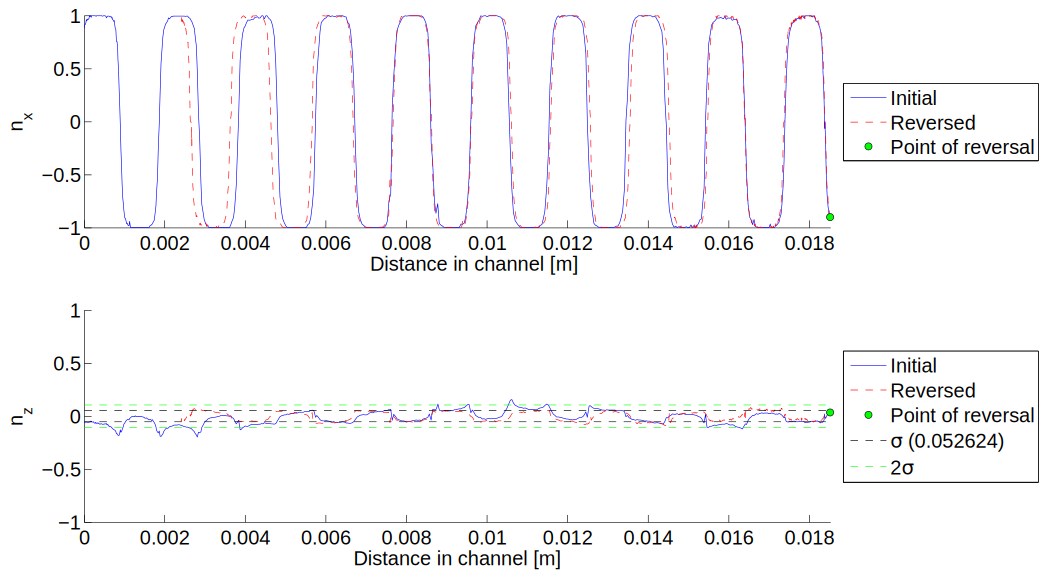
\includegraphics[width=0.7\textwidth]{figures/results/particleA/October_11_Particle_2_run_2_C01.pdf}
\end{center}
\caption{Shows $n_x$ and $n_x$ first and second stretches from Measurement 1, seen in figure \ref{fig:particleA1} but against the actual position in the channel as opposed to cumulative distance. There is an almost perfect match along the entire channel for $n_x$ and only small disagreement for $n_z$. The dashed lines indicate the error margins for detecting $n_z=0$. This figure is the same as can been seen in Laas\cite{alexanderThesis} figure 6.21}
\label{fig:particleAreversegood}
\end{figure}

 \begin{figure}[H]
 \centering
 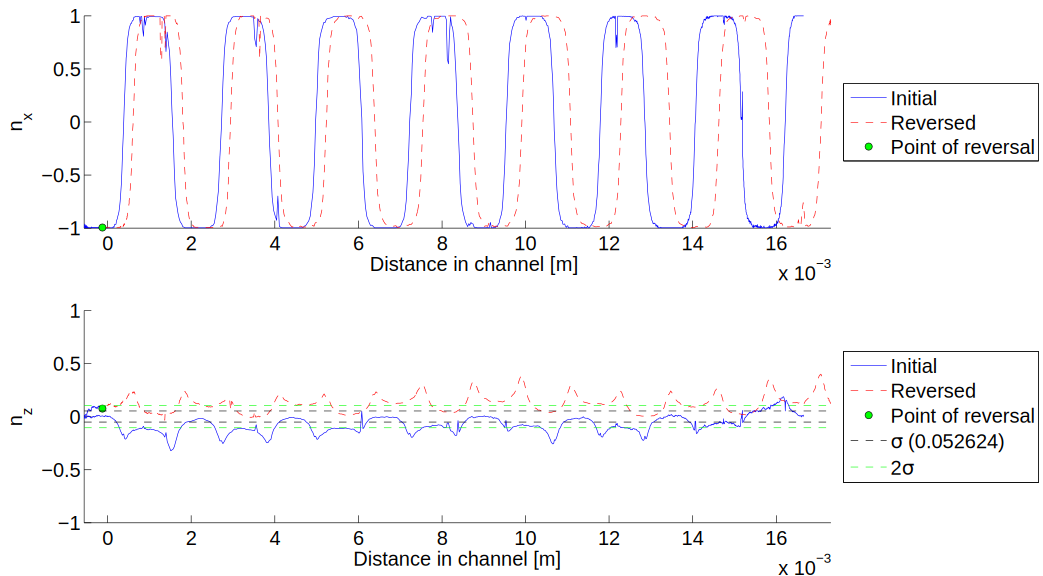
\includegraphics[width=0.8\textwidth]{figures/results/particleA/October_11_Particle_2_run_4_C02.pdf}
 \caption{$n_x$ and $n_z$ from figure \ref{fig:particleA5} for the second and third stretch plotted against actual distance instead of commutative distance. The reversal occurs at the left and although there is some moderate agreement in $n_x$ the match in $n_z$ is non existant from the very start.}
 \label{fig:particleABadReversal}
 \end{figure}
